\begin{figure}
    \centering
    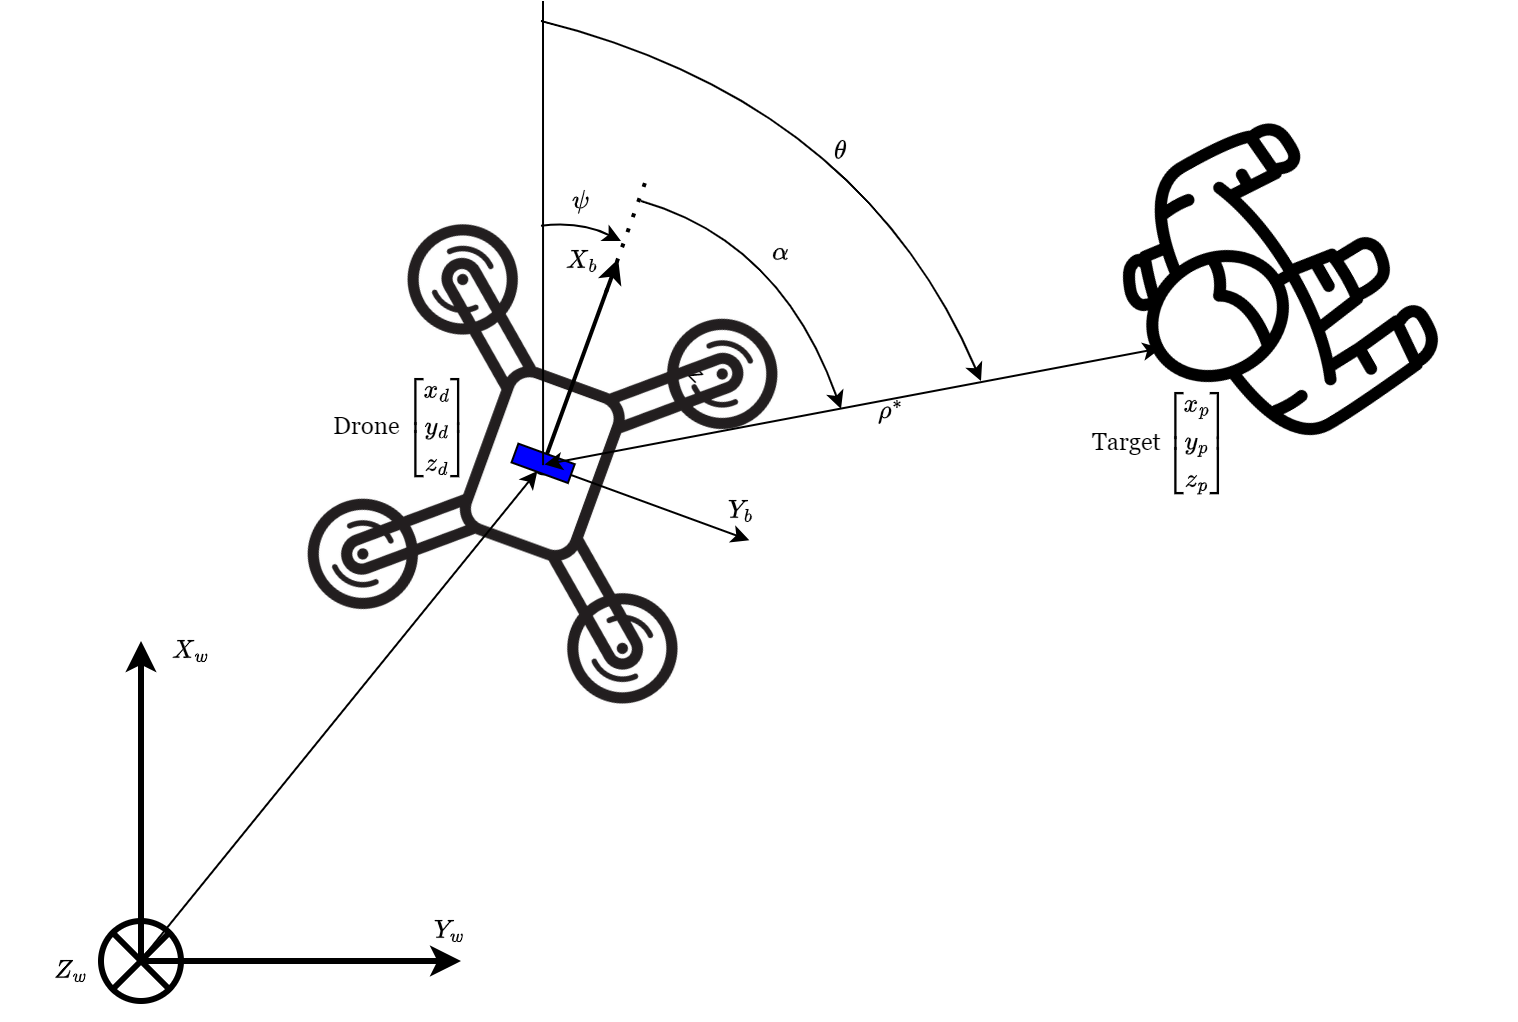
\includegraphics[width=0.47\textwidth]{images/Scheme_drone_tag.png}
    \caption{Application model scheme, in which the actual planar range $\rho^*$, the angles and both the drone local and the global reference frames, are highlighted. In blue is represented the double UWB antenna, deployed perpendicular to the drone's x direction.}
    \label{PRFOR:fig:dronetag_scheme}
\end{figure}


As previously introduced, the problem addressed in this work, is the classical \textit{leader-follower} application using relative range and angle. The policy to be maintained by the follower during the leader motion, is to stay at a constant distance (in the x-y plane), with an AoA of zero. The target (leader) is equipped with the single UWB (i.e. the tag), whereas the quadrotor is equipped with the double UWB (i.e. the follower). Let us define the coordinates of both tag \textbf{p} and follower \textbf{d}, in the fixed global reference frame
\begin{equation}
\textbf{d} = \begin{bmatrix} x_d,y_d,z_d\end{bmatrix}^T \quad , \quad \textbf{p} = \begin{bmatrix} x_p,y_p,z_p\end{bmatrix}^T
\end{equation}
As said, the quantities delivered by the sensor are the range between the two antennas \textbf{$\rho$}, and the angle of arrival of the tag w.r.t. the follower \textbf{$\alpha$}. The range can be expressed as
\begin{equation}
    \rho = ||\mathbf{d} - \mathbf{p}||=\sqrt{(x_d - x_p)^2 + (y_d - y_p)^2 + (z_d - z_p)^2} + \eta = \Bar{\rho} + \eta
\end{equation}
Where $\eta$ is the measure uncertainty, which is supposed to be normally distributed, zero-mean and white, i.e $\eta \sim \mathcal{N}(0,\sigma_{\rho}^2)$. The variance of this quantity, is related to the UWB signal bandwidth and of course with the actual distance $\bar{\rho}$ \cite{uwb_variance}. The range measurement is also affected by a bias introduced by the timestamp delay, which is different for each type of radio and is function of the actual distance $\bar{\rho}$ \cite{UWBEvaluationOP}. Since in the proposed application the measured distance (without considering the initial conditions), should stay in a relatively strict band, a calibration in that zone of interest, should be enough to mitigate the bias. Given that, the bias is supposed to be negligible. In the end, Line-of-sight (LOS) and negligible shadowing conditions are assumed, and so also Non-line-of-sight and shadowing sources of error \cite{UWBHumshadowing}, are neglected.\\
Clearly the measure obtained is the pure 3D range which is not the wanted quantity, since the described policy is to maintain a certain distance in x-y plane. With the described configuration, it is not possible to directly obtain this value. But if we suppose that the quadrotor can collects measurements about its height $h$ w.r.t. to the ground (e.g. with a distance sensor, or any type of global positioning system) and assuming a fixed known value for the target height, it is possible to calculate the projection of the range in the x-y plane $\rho^*$. The assumption about the target height, can be simply made by knowing at which height the tag will be kept. Since in our test the tag is placed on a ground robotic agent, we have simply measured the height and saved it as the constant $h_t$. In the end the projection $\rho^*$ can be calculated as follow:
\begin{equation}
    \rho^* = \sqrt{\rho^2 - \big( z_d - h_t\big)^2}
\end{equation}
where the double UWB antenna height $z_d = z + h_d$, i.e. the sum of the quadrotor height estimates $z$ and the relative height of the double antenna w.r.t. the flight controller $h_d$ (which is a construction constant).\\

For what concerns the angle of arrival, if we consider the double UWB face placed perpendicular to the x drone axis (as depicted in \autoref{PRFOR:fig:dronetag_scheme}) , it is possible to define the angle of arrival \textbf{$\alpha$} measured by the UWB, as follow:
\begin{equation}
    \alpha = \theta -\psi+ \xi
\end{equation}
where $\psi$ is the yaw orientation of the quadrotor, $\theta$ is the geometric angle between the follower and the tag in the x-y plane and $\xi$ is the measure uncertainty, which, as for the range, is supposed to be normally distributed, zero-mean and white, that is $\xi \sim \mathcal{N}(0,\sigma_a^2)$. The same considerations and assumptions done for the range uncertainty, are also valid for the angle uncertainty. This angle is obtained from the PDoA, that is the difference in phase of the signal received by the two antennas of the follower, by means of the following relation:
\begin{equation}\label{PRFOR:eq:aoa-pdod}
    \alpha = \arcsin \Bigg( \frac{\Delta\phi \cdot \lambda}{2\pi\cdot d} \Bigg)
\end{equation}
where $\Delta\phi$ is the PDoA, $\lambda$ is the signal wavelength and $d$ is the wheelbase between the two, in the double UWB, antennas. This conversion from PDoA to AoA is performed directly inside the Nordic companion board of the antenna, given that all the constant like $\lambda$ and $d$ are given in construction phase. Moreover, as will be later explained, this conversion is performed by knowing the calibration PDoA offset and the number of elements averaging it. Both those quantities can be modified from serial port, to obtain the better possible value in the calibration phase.

\subsection{Control law}\label{control_law}
Let us define the wanted policy, as a vector with the wanted range, angle and height $r_w = \begin{bmatrix} \rho_w, \alpha_w, z_w \end{bmatrix}^T$ and the estimated range, angle and height at time t $r_a(t) = \begin{bmatrix} \rho^* (t) , \alpha(t), z(t) \end{bmatrix}^T$. The control law has the scope of minimizing and maintaining low the difference $r_a - r_W$ in time. To do so three different control strategies are implied:
\begin{itemize}
    \item a PID controller to generate the x-y velocities setpoints
    \item a setpoint control for the yaw
    \item a setpoint control for the height
\end{itemize}
The PID controller is based on the difference between the actual measured range $\rho^*$ and the wanted value $\rho_w$, and by defining $d = \rho^* - \rho_w$, a scalar control value $V_s$ can be calculated:
\begin{equation}
    V_{s_k} = K_p\cdot d_k + K_d\cdot\Big(\frac{d_k - d_{k-1}}{\Delta t}\Big) + K_i\cdot I_{d_k}\Delta t
\end{equation}
Where $K_p$, $K_d$, $K_i$ are the proportional, derivative and integral gain respectively, $\Delta t$ is the time-step and $I_d$ is the cumulative integral value which can be defined as follow:
\[
    I_{d_k} = I_{d_{k-1}} + d_k
\]
The subscript $k$ defines the discrete $k$ instant at which the control is calculated. In order to obtain the actual x-y pair velocities, a last projection step has to be performed. Since the quantity $V_{s_k}$ represents the velocity to be applied in the direction of the target, the $V_{x_k}$ and $V_{y_k}$ control velocity, expressed in the global frame, can be obtained as follow:
\begin{equation}\label{PF:VELxy}
    \begin{bmatrix} V_{x_k} \\ V_{y_k} \end{bmatrix} = V_{s_k} \cdot \begin{bmatrix} \cos (\theta_k) & \sin (\theta_k) \end{bmatrix}^T
\end{equation}
where $\theta_k$, as already mentioned, is the geometric planar angle between the target and the drone and can be derived as:
\begin{equation}\label{PF:yawsp}
    \theta_k = \alpha_k +\psi_{k_{estim}}
\end{equation}
where $\psi_{k_{estim}}$ is the quadrotor yaw angle, estimated by the flight controller. Obviously this quantity is affected by both the uncertainty of the AoA measure $\alpha_k$ and of $\psi_{k_{estim}}$.\\
The two obtained control velocities, are fed to the flight controller as a velocity setpoint $V_{sp} = \begin{bmatrix} V_{x_k}, V_{y_k}, * \end{bmatrix}$, whereas $\theta$ is fed as the yaw setpoint, $\psi_{sp}$, to orient the drone toward the target. Lastly the height is controlled by feeding the flight controller with a position setpoint, $X_{sp} = \begin{bmatrix} *, *, z_w \end{bmatrix}$\footnote{The * simply means that the quantity is not given so not controlled}.
